\section{Experiments}
\label{sec:experiment}

\begin{table*}[th!]
	\centering
	\scriptsize
	\begin{tabular}{l|lccc}
		\toprule
		\textbf{Dataset} &\textbf{Premise}  & \textbf{Choices} & \textbf{Training size} & \textbf{Test size}\\
		\midrule
		\makecell[c]{ROC} &  \makecell[l]{Sarah was home alone.\\She wanted to stay busy.\\She turned on the TV.\\She found a reality show to watch.} &\makecell[l]{Sarah then happily watched the show.     \checksymbol 
		\\Sarah could not find anything to watch. \crosssymbol }&\makecell[c]{1871}&\makecell[c]{1871}\\
		\midrule
		\makecell[c]{ARCT} &\makecell[l]{\textbf{Reason}: Milk isn’t a gateway drug even though \\ most people drink it as children. \\\textbf{Claim}: Marijuana is not a gateway drug.}&\makecell[l]{\textbf{Warrant 1}: Milk is similar to marijuana. \checksymbol \\
		\textbf{Warrant 2}: Milk is not marijuana.\crosssymbol}&\makecell[c]{1210}&\makecell[c]{444}\\
		\midrule
		\makecell[c]{RECLOR} &\makecell[l]{\textbf{Context}:In a business...to financial prosperity. \\
		\textbf{Question}:The reasoning in the argument\\  is flawed because the argument}&\makecell[l]{A: ignores the fact that in... the family 's prosperity.\checksymbol
		\\B: presumes, without... the family's prosperity.\crosssymbol
		\\C: ignores the fact... even if they pay high wages.\crosssymbol
		\\D: presumes, without providing...can succeed.\crosssymbol}&\makecell[c]{4638}&\makecell[c]{500}\\
		
		
		\bottomrule
	\end{tabular}
	\caption{Examples for three other datasets.}
	\label{table:dataset}
\end{table*}


First, we show the experimental setup. 
Second, we compare several test operators for the discovery of short circuit problems. 
Third, we evaluate robustness and the ability to avoid short circuit 
for models with different augmentation methods.

\subsection{Experimental Setup}
\label{sec:setup}

In this section, we will present our experimental setup, including the datasets, models, and test operators used in our study.

\subsubsection{Datasets}

We experiment on four datasets from four different tasks:

\textbf{ROC} is a story ending prediction dataset. The task is to identify the correct ending of a four-sentence story premise from two alternative choices. An example is shown in~\tabref{table:dataset}.

\textbf{COPA} is a causal reasoning dataset, an example of which was previously shown in~\secref{sec:intro}. Given a premise context, COPA requires choosing the more plausible, causally related choice. There are 500 instances in the training data and 500 instances for testing.

\textbf{ARCT} is an argument reasoning comprehension dataset. It contains questions where the reason is connected to the claim, and there may exist an alternative warrant choice.

\textbf{RECLOR} is a reading comprehension dataset that requires logical reasoning to answer questions based on provided text passages.

\subsubsection{Models}

We mainly investigate three popular classifiers based on pre-trained language models. There are several available versions of pre-trained models differing in the number of layers and parameters. We choose to use the base version of each model. We train and test all the models on a server with a GeForce GTX 1080 Ti GPU with 11G RAM and an Intel(R) Xeon(R) CPU E5-2630 with 128G of RAM.

\textbf{BERT} (BT) is a popular attention model that applies the bidirectional training of the Transformer architecture. The base version has 12 Transformer layers, a hidden size of 768, and 12 self-attention heads, totaling 110M parameters. It is fine-tuned for three epochs to predict the relation based on context and choices.

\textbf{XLNet} (XL) is an autoregressive pre-trained language model that combines the strengths of BERT with the permutation-based training approach. It introduces a new technique called Permutation Language Modeling, which enables the model to learn bidirectional context by maximizing the expected likelihood over all possible permutations of the input sequence. XLNet does not use the Next Sentence Prediction (NSP) objective as BERT does.

\textbf{RoBERTa} (RB) is an improved pre-training procedure of BERT that involves training the model on more data, using larger batch sizes, and removing the NSP objective. These changes result in a more robust and better-performing model compared to the original BERT architecture.

\subsubsection{Stress Test Cases}

Following previous research~\cite{checklist2020acl}, 
we will test the effectiveness of different data augmentation
methods by looking at the robustness of models against
different stress tests.
We create these stress test cases using the proxy operations
introduced in \tabref{table:proxyop}.
Different operations generate different number of cases,
as shown in \tabref{tab:cases}. To evaluate the
ability to test for short-circuiting, we will
use a subset of these test cases in the next section. 



\begin{table}[th]
\centering
\scriptsize
\begin{tabular}{c|rrrr}
\toprule
\textbf{Stress} & \textbf{ROC} & \textbf{COPA} & \textbf{ARCT} & \textbf{RECLOR} \\ \midrule
Neg+  &	1,797&492&	297&375	\\ \hline
Neg-  &	94&	2&	152&	119\\ \hline
NER  &	362&	0&	5&0	\\ \hline
PR  &	1,073&	328&71&72	\\ \hline
PI  &	     861&	219&	56&	91\\ \midrule
Adv  &	1,850&496	&444	&500	\\ \hline
CO  &	1,871&500	&444	&500	\\ \hline
Syn&	653&	 25&	303&289	\\ \midrule
MT  &	1,871&500	&444	&500	\\ \hline
Voice  &	1,014&246	&174	&263	\\ \hline
Total & 11,446  &  2,808 & 2,390 & 2,709 \\ \bottomrule
\end{tabular}
\caption{Number of stress test cases by different operations for 4 datasets.}
\label{tab:cases}
\end{table}
\subsection{Testing for Short Circuit}
\label{sec:short_circuit}

In this section, we will select proper testing operators for short circuit testing, and use these operators to detect the extent of model short circuiting.

\subsubsection{Selecting Short Circuit Testing Methods}
\label{sec:select-sc}

In~\secref{sec:proxy}, we discussed the possibility that both white-box 
attention-based method (AW~\footnote{Here, $t\_1$ and $t\_2$ are tuned to 0.14 and 0.13 respectively, using 100 human-labeled cases. These cases are randomly sampled from the training data across the four datasets.}) 
and black-box choice operators in some 
of the equivalent classes can evaluate 
short circuits. We now investigate which proxy tests are better suited for short circuit evaluation.

As described in \secref{sec:proxy}, each test operator generates new test cases 
by making directional changes to the test cases that the model 
chooses the right answer. The model is considered not short-circuiting 
on a case according to a test operator if it still gets the 
right answer after the operation. Assuming that human attention 
annotation, attention weight thresholding, and each choice 
operator are all plausible proxy tests, we can obtain 9 
different proxy tests. 

Then, we randomly sample 30 MCQs 
from the test set of ROC that are correctly answered 
by three models, respectively. Each proxy test will 
produce a 30-dimensional one-hot vector (proxy vector) 
for each model, where 1/0 indicates if the model 
short-circuited on that specific MCQ or 
not\footnote{For MCQs where a certain proxy test is not applicable, we randomly label it as 1 or 0.}. 
For each model, we then compute another vector as the ensemble of all 
proxy tests by majority voting on each of the 30 dimensions. 

The smaller Euclidean distance between the individual 
proxy vector of each test type and the ensemble vector 
indicates higher reliability. The full results are shown in \tabref{tab:agree}. We can find that the results of CO and AW are generally closer to the ensembled results, as reflected by the smaller distances. Thus, we consider that CO and AW are more suitable as proxy tests for short circuit evaluation.

%It is worth noting that we do not use human labeling results on attention maps as gold indicators. Because the attention map on each model is not a direct expression of the final decision for multiple-choice questions, but the expression of the premise and choices, which is an indirect information for reasoning.

\begin{table}[th]
\scriptsize
\centering
\begin{tabular}{c|cccc}\hline
\toprule  
\textbf{Test types} &BERT  & XLNet & RoBERTa  &Ave\\ 
 \midrule
{Neg+}      &     3.16	&3.87&	\textbf{2.45}	&3.16\\
\midrule
{Neg-}&    3.74&3.74&	4.12&	3.87\\
\midrule
{NER}    &    3.87&	3.87	&4.12	&3.95\\
\midrule
{PR}&   4.0&	3.61&	3.87	&3.83\\
\midrule
{PI}&    3.74	&3.74&	3.74&	3.74\\
\midrule
{CO}            & \textbf{ 2.83}	&\textbf{2.63}	&2.83	&\textbf{2.76}\\
\midrule
{AW}   &  \textbf{2.45}	&3.46&	\textbf{2.45}	&\textbf{2.79} \\
\midrule
{Choice-only}   &     4.0&	3.74&	3.87&	3.87\\
\midrule
{Human}   &3.0&	\textbf{2.55}&	3.0&	2.85\\
\bottomrule
\hline
\end{tabular}
\caption{\label{tab:agree} 
Euclidean distances between proxy vector and 
the ensemble vector on short circuit test (the smaller
the better). 
Ave is the average score across all models.
Top two tests for each model are highlighted.}
\end{table}

\subsubsection{Testing Short Circuit Problems}
\label{sec:fix-sc}
We test short circuits by observing AW and CO scores, i.e., higher AW/CO scores indicate a lower chance for short-circuiting. We fine-tune the multiple-choice classifiers of BERT, XLNet, and RoBERTa on four datasets. In~\tabref{tab:results}, we observe that the original models (in gray color) without data augmentation are most susceptible to short-circuits, as the AW and CO scores are relatively low. For the XLNet model on ROC, the AW score is even lower than 30\%, which suggests a high likelihood of short-circuiting on ROC.


\begin{table*}[th!]
\small
\centering
\begin{subtable}[t]{0.48\textwidth}
\centering
\begin{tabular}{l|cc|cc}\toprule
	& \multicolumn{2}{c|}{\bf Short circuit Tests} & \multicolumn{2}{c}{\bf Robustness Tests} \\ \cline{2-5}
\textbf{Model} &\textbf{AW} &\textbf{CO} & \textbf{Original} &\textbf{Stress}\\ \hline
\rowcolor{Gray}
BT(w/o)&98.76&90.80&86.58&81.93\\
BT+B&99.26&92.54&86.75&82.96\\
BT+C&\textbf{99.69}&\textbf{98.47}&\textbf{87.07}&84.34\\
BT+M&99.26&91.47&86.48&86.06\\
BT+C+M&98.82&97.78&86.75&\textbf{88.60}\\
\midrule

\rowcolor{Gray}
XL(w/o)&28.08&83.28&\textbf{90.81}&79.22\\
XL+B&19.27&84.4&90.43&82.23\\
XL+C&\textbf{64.58}&\textbf{98.81}&89.47&86.23\\
XL+M&62.77&86.90&90.17&89.47\\
XL+C+M&60.25&97.10&90.22&\textbf{92.64}\\
 \midrule
\rowcolor{Gray}
RB(w/o)&77.41&88.76&\textbf{92.73}&82.33\\
RB+B&58.15&87.98&92.46&78.50\\
RB+C&82.71&\textbf{99.3}&91.18&88.92\\
RB+M&71.73&88.06&92.62&90.29\\
RB+C+M&\textbf{93.31}&97.44&91.88&\textbf{93.06}\\
\bottomrule
\end{tabular}
\caption{ROC}
\end{subtable} 
\hfill
\begin{subtable}[t]{0.48\textwidth}
\centering
\begin{tabular}{l|cc|cc}\toprule
	& \multicolumn{2}{c|}{\bf Short circuit Tests} & \multicolumn{2}{c}{\bf Robustness Tests} \\ \cline{2-5}
\textbf{Model} &\textbf{AW} &\textbf{CO} & \textbf{Original} &\textbf{Stress}\\ \hline
\rowcolor{Gray}
BT(w/o)&89.68&68.71&62.00&57.40\\
BT+B&96.79&85.42&68.60&68.95\\
BT+C&\textbf{98.35}&\textbf{97.25}&\textbf{72.80}&78.84\\
BT+M&95.17&90.62&70.40&79.62\\
BT+C+M&96.69&96.13&72.40&\textbf{80.68}\\
\midrule
                     
\rowcolor{Gray}
XL(w/o)&93.16&60.26&61.40&57.71\\
XL+B&91.46&65.51&63.20&61.06\\
XL+C&45.13&\textbf{94.69}&\textbf{67.80}&75.42\\
XL+M&76.85&57.23&62.20&71.10\\
XL+C+M&\textbf{98.51}&83.93&67.20&\textbf{81.32}\\

\midrule

\rowcolor{Gray}
RB(w/o)&80.89&78.01&76.40&74.85\\
RB+B&\textbf{96.36}&83.64&77.00&80.26\\
RB+C&89.62&\textbf{98.23}&\textbf{79.00}&83.31\\
RB+M&62.26&84.30&72.60&83.53\\
RB+C+M&61.89&92.70&74.00&\textbf{87.30}\\
\bottomrule
\end{tabular}
\caption{COPA}
\end{subtable} 
\hfill
\begin{subtable}[t]{0.48\textwidth}
\centering
\begin{tabular}{l|cc|cc}\toprule
	& \multicolumn{2}{c|}{\bf Short circuit Tests} & \multicolumn{2}{c}{\bf Robustness Tests} \\ \cline{2-5}
\textbf{Model} &\textbf{AW} &\textbf{CO} & \textbf{Original} &\textbf{Stress}\\ \hline
\rowcolor{Gray}
BT(w/o)&\textbf{99.65}&78.52&63.96&58.08\\
BT+B&99.34&61.18&68.47&56.21\\
BT+C&98.37&\textbf{96.08}&\textbf{68.92}&65.73\\
BT+M&98.67&74.42&67.79&69.65\\
BT+C+M&98.00&90.0&67.57&\textbf{73.71}\\
\midrule
                   
\rowcolor{Gray}
XL(w/o)&85.67&59.10&75.45&61.72\\
XL+B&95.73&60.40&\textbf{79.05}&64.78\\
XL+C&55.59&\textbf{92.45}&74.55&69.93\\
XL+M&\textbf{95.74}&59.57&74.10&73.15\\
XL+C+M&86.26&90.35&77.03&\textbf{79.11}\\
\midrule

\rowcolor{Gray}
RB(w/o)&99.14&60.29&78.83&66.16\\
RB+B&97.78&60.94&\textbf{81.31}&66.02\\
RB+C&79.19&92.77&77.93&70.64\\
RB+M&\textbf{100.00}&68.13&77.03&76.64\\
RB+C+M&71.47&\textbf{93.39}&75.00&\textbf{78.97}\\
\bottomrule
\end{tabular}
\caption{ARCT}
\end{subtable} 
\hfill
\begin{subtable}[t]{0.48\textwidth}
\centering
\begin{tabular}{l|cc|cc}\toprule
	& \multicolumn{2}{c|}{\bf Short circuit Tests} & \multicolumn{2}{c}{\bf Robustness Tests} \\ \cline{2-5}
\textbf{Model} &\textbf{AW} &\textbf{CO} & \textbf{Original} &\textbf{Stress}\\ \hline
\rowcolor{Gray}
BT(w/o)&82.46&50.88&45.60&33.91\\
BT+B&86.01&61.73&\textbf{48.60}&35.99\\
BT+C&80&\textbf{96.17}&47.00&47.72\\
BT+M&82.48&58.55&46.80&50.02\\
BT+C+M&\textbf{96.79}&87.16&43.60&\textbf{53.79}\\
\midrule
                 
\rowcolor{Gray}
XL(w/o)&79.64&62.86&56.00&39.77\\
XL+B&81.40&74.04&\textbf{57.0}&44.6\\
XL+C&\textbf{87.87}&\textbf{98.90}&54.40&51.66\\
XL+M&72.76&70.15&53.60&56.99\\
XL+C+M&48.71&88.56&54.2&\textbf{58.63}\\
\midrule
\rowcolor{Gray}
RB(w/o)&85.88&70.2&51.00&36.76\\
RB+B&15.69&73.73&51.00&38.71\\
RB+C&89.68&\textbf{96.83}&50.40&50.88\\
RB+M&\textbf{100.00}&80.38&\textbf{52.00}&\textbf{59.95}\\
RB+C+M&89.26&88.43&48.40&55.78\\
\bottomrule
\end{tabular}
\caption{RECLOR}
\end{subtable}
\caption{\label{tab:results} Short circuit and Robustness Tests
on 4 models with or without(w/o) data augmentation. 
+B = augmented with back-translation,
+C = augmented with crossover, +M = augmented with mutation, 
CO=crossover, AW=attention weight evaluation. 
Stress includes all cases in \tabref{tab:cases}.}
%Robustness Test includes: Neg+=negation-add, Neg-=negation-remove, NER, 
%PR=pronoun-replacement, PI=Pronoun-instantiation, Adv=adverbial, MT=mutation, Voice, Syn=synonym.}

\end{table*}

\subsection{Improving Overall Model Robustness}
\label{sec:robust}
To address the issue of model robustness, we tested the models and proposed data augmentation methods to improve their performance. Our analysis reveals that BERT, XLNet, and RoBERTa models on various datasets are generally not robust under stress tests. To remedy this, we employed data augmentation techniques, such as crossover, mutation, and a combination of both (+C+M), and compared their effectiveness to a back-translation baseline.

\subsubsection{Model Weakness}
As shown in Table~\ref{tab:results}, BERT, XLNet, and RoBERTa models exhibit a significant performance drop when subjected to stress tests. For instance, the accuracy rate of the XLNet model trained with ROC declines by 11.59\%, and the AW short circuit score is 28.8\%, suggesting that the model may be susceptible to short circuit issues. Similarly, all three models perform worse on the RECLOR and ARCT datasets, with a performance drop of about 10\%, which aligns with the lower CO scores. These results indicate that model instability is a widespread problem, and short circuit is a probable cause. For more details on the stress test results, please refer to the Appendix.

\subsubsection{Data Augmentation}
To mitigate the weaknesses identified, we trained models using two primary data augmentation methods: crossover and mutation, which were discussed in the previous section. We also combined these two methods (+C+M) by constructing training data that incorporates both techniques. We used back-translation~\cite{back2019} as the baseline for data augmentation, as it has demonstrated universality and effectiveness in previous work. The expanded data volume is consistent with the original data volume.

Table~\ref{tab:results} presents the results for the``original test.'' We observe that the four data augmentation methods do not negatively impact the model's performance on the original dataset and may even help the model achieve better accuracy. For instance, in the ROC dataset, the accuracy of BERT and RoBERTa models trained with crossover augmented data surpasses the base model, ranking first. The crossover method also proves effective on COPA. Although back-translation mostly achieves higher scores on ARCT and RECLOR, +C, +M, and +C+M methods only slightly underperform compared to the base model.

Considering the``Stress'' column in Table~\ref{tab:results}, we find that different methods exhibit varying levels of robustness. Overall, the +C+M method demonstrates the best performance on the stress test, except when training RoBERTa on the RECLOR dataset. This outcome indicates that this type of data can protect models from confusion caused by simple perturbations and enhance model robustness. However, back-translation does not significantly improve model robustness. While the crossover method alone can contribute to robustness under stress tests, it is not as effective as +M and +C+M methods.

Further analysis of the models using the short circuit test reveals that the crossover method consistently achieves the highest CO score and often ranks best in the AW score. This finding suggests that models trained with crossover data augmentation learn to consider the premise to avoid short circuit issues.

\subsubsection{Results}
In conclusion, our study demonstrates the importance of addressing model robustness and short circuit issues when developing machine learning models for natural language understanding tasks. By investigating the weaknesses of BERT, XLNet, and RoBERTa models across different datasets, we identified that these models are generally not robust under stress tests, and short circuit issues contribute to their instability.

To overcome these challenges, we proposed and evaluated data augmentation methods, including crossover, mutation, and a combination of the two (+C+M), and compared them with the back-translation baseline. Our results revealed that these data augmentation techniques not only maintain or improve the model's performance on the original dataset but also significantly enhance model robustness under stress tests. In particular, the +C+M method demonstrated the best performance for most of the cases.

Additionally, our findings from the short circuit test showed that the crossover method consistently achieves the highest CO score and often ranks best in the AW score, indicating that models trained with crossover data augmentation are more likely to consider the premise and avoid short circuit issues.

Future work could explore additional data augmentation techniques and their combinations to further enhance model robustness and mitigate short circuit problems. Furthermore, investigating the transferability of these augmentation methods across various natural language understanding tasks and languages could provide valuable insights into the generalizability of these approaches.


\subsection{Case Study}
\label{sec:case}

Our case study is a series of white-box tests that demonstrate
the change in attention patterns.

We take an example from ROC which is shown in~\tabref{table:dataset}.
We explore BERT-based models by 
analyzing their attention maps on this case in~\figref{fig:roc_bert}.  
In this example, the word ``show'' in the premise is strongly
related to the token ``reality show'' in the right choice from human knowledge. 
%The relationship between these two words is the key to answering this question. 
%We explore different models with the augmentation method with attention map 
%to visualize if these two words have a relationship or not.
%The attention map is visualized via an off-the-shelf tool~\cite{vig-2019-multiscale}.


There is no positive attention value in front of the fourth sentence, 
so we intercept it from where it is worth. 
BERT trained on the original training set fails 
to pick up the right choice likely due to there being 
virtually no attention connection between words in 
the choice and words in the premise.
After training with \textit{crossover} data augmentation, 
the model learns  
to pay attention to the premise and the relationship 
between premise and choices. 
i.e., ``show'' in this example. 
Similar trends also exist for the \textit{mutation} operation in \figref{fig:roc_bert} (``BT+M'')
and the combination of \textit{crossover} 
and \textit{mutation} operation in~\figref{fig:roc_bert} (``BT+C+M''). 
The rationale behind 
such a change of attention pattern is that, 
in an MCQ created by \textit{crossover} operation (``BT+C'' in \figref{fig:roc_bert}), 
\textit{mutation}(``BT+M'' in \figref{fig:roc_bert}), 
and the combination of them (``BT+C+M'' in \figref{fig:roc_bert}), 
the model needs to combine the information 
in the premise to effectively 
distinguish the true ``right'' choice from the wrong one. 
However, the light and sparse attention color blocks on the attention map for back-translation 
in \figref{fig:roc_bert} (``BT+B'') indicate back-translation 
can not help BERT connect the choice and premise very well in this question.
These observations empirically demonstrate the effectiveness of our methods 
in encouraging the model to pay attention to the premise to reduce 
short circuits. 


\begin{figure}[h!]
\centering
\begin{minipage}{0.45\linewidth}
    \centering
    \fbox{\includegraphics[width=\linewidth]{figure/roc_b.eps}}
    \caption*{BT+B}
    \label{fig:roc_b}
\end{minipage}
\hspace{0.5cm}
\begin{minipage}{0.45\linewidth}
    \centering
    \fbox{\includegraphics[width=\linewidth]{figure/roc_c.eps}}
    \caption*{BT+C}
    \label{fig:roc_c}
\end{minipage}
\hspace{1.5cm}
\vspace{0.5cm}
\begin{minipage}{0.45\linewidth}
    \centering
    \fbox{\includegraphics[width=\linewidth]{figure/roc_m.eps}}
    \caption*{BT+M}
    \label{fig:roc_m}
\end{minipage}
\hspace{0.5cm}
\begin{minipage}{0.45\linewidth}
    \centering
    \fbox{\includegraphics[width=\linewidth]{figure/roc_cm.eps}}
    \caption*{BT+C+M}
    \label{fig:roc_cm}
\end{minipage}
\caption{Attention map on a ROC example for BERT-based models.}
\label{fig:roc_bert}
\end{figure}



